%%%%%%%%%%%%%%%%%%%%%%%%%%%%%%%%%%%%%%%%%
% Short Sectioned Assignment
% LaTeX Template
% Version 1.0 (5/5/12)
%
% This template has been downloaded from:
% http://www.LaTeXTemplates.com
%
% Original author:
% Frits Wenneker (http://www.howtotex.com)
%
% License:
% CC BY-NC-SA 3.0 (http://creativecommons.org/licenses/by-nc-sa/3.0/)
%
%%%%%%%%%%%%%%%%%%%%%%%%%%%%%%%%%%%%%%%%%

%----------------------------------------------------------------------------------------
%	PACKAGES AND OTHER DOCUMENT CONFIGURATIONS
%----------------------------------------------------------------------------------------

\documentclass[letterpaper, fontsize=11pt]{scrartcl} % A4 paper and 11pt font size

\usepackage[T1]{fontenc} % Use 8-bit encoding that has 256 glyphs
\usepackage{fourier} % Use the Adobe Utopia font for the document - comment this line to return to the LaTeX default
\usepackage[english]{babel} % English language/hyphenation
\usepackage{amsmath,amsfonts,amsthm} % Math packages

\usepackage{lipsum} % Used for inserting dummy 'Lorem ipsum' text into the template
\usepackage[margin=1in]{geometry} %set margins -TA
\usepackage{sectsty} % Allows customizing section commands
\allsectionsfont{\centering \normalfont\scshape} % Make all sections centered, the default font and small caps
\usepackage{enumitem}
\usepackage{fancyhdr} % Custom headers and footers
\usepackage{graphicx}
\pagestyle{fancyplain} % Makes all pages in the document conform to the custom headers and footers
\fancyhead{} % No page header - if you want one, create it in the same way as the footers below
\fancyfoot[L]{\textit{CME 102 Spring '15-'16}} % Empty left footer
\fancyfoot[C]{} % Empty center footer
\fancyfoot[R]{Tim Anderson} % Page numbering for right footer
\renewcommand{\headrulewidth}{0pt} % Remove header underlines
\renewcommand{\footrulewidth}{0pt} % Remove footer underlines
\setlength{\headheight}{14pt} % Customize the height of the header


\usepackage{mdframed}
\usepackage{caption}
\usepackage{subcaption}
\usepackage{float}
\usepackage{array}
\usepackage{soul}
\usepackage{amsmath}
\usepackage{graphicx} % Required to insert images
\usepackage{multicol}
\usepackage{enumitem}
\usepackage{amssymb}
\usepackage{bm}
\usepackage{verbatim}
\usepackage{hyperref}

\allowdisplaybreaks

\numberwithin{equation}{section} % Number equations within sections (i.e. 1.1, 1.2, 2.1, 2.2 instead of 1, 2, 3, 4)
\numberwithin{figure}{section} % Number figures within sections (i.e. 1.1, 1.2, 2.1, 2.2 instead of 1, 2, 3, 4)
\numberwithin{table}{section} % Number tables within sections (i.e. 1.1, 1.2, 2.1, 2.2 instead of 1, 2, 3, 4)

\setlength\parindent{0pt} % Removes all indentation from paragraphs - comment this line for an assignment with lots of text
\begin{document}

%----------------------------------------------------------------------------------------
%	TITLE SECTION
%----------------------------------------------------------------------------------------

\newcommand{\horrule}[1]{\rule{\linewidth}{#1}} % Create horizontal rule command with 1 argument of height

%----------------------------------------------------------------------------------------
%	PROBLEM 1
%----------------------------------------------------------------------------------------

\section*{Laplace Transform Review Solutions}

\begin{enumerate}
\item Find the Laplace transform for the following functions. If an image is given, first write out the function and then take the transform.

\begin{enumerate}

\item $e^{-t}\sinh (4t)$
\par \textbf{Solution:}
\par From \#8 on the table: $$\mathcal{L}\{\sinh(4t)\} = \frac{4}{s^2 - 16}$$
Using \#12 on the table: 
$$\mathcal{L}\{e^{at}f(t)\} = Y(s-a) \implies \mathcal{L}\{e^{-t}\sinh(4t)\} = \frac{4}{(s+1)^2 - 16}\quad\blacksquare$$

\item $1.5\sin(3t-\pi/2)$
\par \textbf{Solution:}
\begin{align*}
f(t) &= 1.5\sin(3t - \pi/2)\\
&= 1.5\sin(3t)\cos(\pi/2) - 1.5\sin(\pi/2)\cos(3t)\\
&= -1.5\cos(3t)\\
\mathcal{L}\{f(t)\} &= -1.5\frac{s}{s^2 + 9} \quad\blacksquare
\end{align*}
Note: we do not use \#13 from the table ($t$-shift) because $f(t)$ is not multiplied by a Heaviside step function.

\item Function given in the following figure:
\begin{figure}[H]
\centering 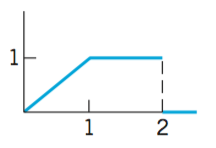
\includegraphics[width = 0.3\columnwidth]{LaplaceFig1.png}
\end{figure}
\end{enumerate}
\par \textbf{Solution:}
\par Whenever you're given an image that you need to find the transform of, it is first helpful to write it as a piecewise function, and then transform this piecewise function into a ``single-line" form with Heaviside step functions we can take the Laplace transform of:
\[
f(t) = \begin{cases}
t & 0< t < 1\\
1 & 1< t< 2\\
0 & t > 2
\end{cases}
\]
Now we can multiply each part of the piecewise function with a boxcar function to ``window" that part of the piecewise function to only its relevant interval:
$$f(t) = (1 - u(t-1))t + (u(t-1) - u(t-2))$$
Finally, we should rearrange this to be in a form such that we can apply \#13 from the table ($t$-shift):
\begin{align*}
f(t) &= (1 - u(t-1))t + (u(t-1) - u(t-2))\\
&= t - tu(t-1) + (u(t-1) - u(t-2))\\
&= t - (t-1+1)u(t-1) + (u(t-1) - u(t-2))\\
&= t - ((t-1)+1)u(t-1) + (u(t-1) - u(t-2))\\
&= t - (t-1)u(t-1)-u(t-1) + u(t-1) - u(t-2)\\
&= t - (t-1)u(t-1) - u(t-2)\\
\mathcal{L}\{f(t)\} &= \frac{1}{s^2} - \frac{e^{-s}}{s^2} -\frac{e^{-2s}}{s} \quad\blacksquare
\end{align*}

\item Solve the following initial value problems:
\begin{enumerate}
\item $y'' + 9y = 10e^{-t},\quad y(0) = y'(0) = 0$
\par \textbf{Solution:}

\begin{align*}
y'' + 9y &= 10e^{-t}\\
s^2Y(s) - sy(0) - y'(0) + 9Y(s) &= \frac{10}{s+1}\\
\intertext{Apply initial conditions:}
s^2Y(s) + 9Y(s) &= \frac{10}{s+1}\\
Y(s)(s^2 + 9) &= \frac{10}{s+1}\\
Y(s) &= \frac{10}{(s+1)(s^2 + 9)}
\end{align*}
Now we need to do a partial fraction decomposition:
\begin{align*}
\frac{10}{(s+1)(s^2 + 9)} &= \frac{A}{s+1} + \frac{Bs + C}{s^2 + 9} \\
10 &= A(s^2 + 9) + Bs(s+1) + C(s+1)\\
&= As^2 + 9A + Bs^2 + Bs + Cs + C\\
&= s^2(A+B) + s(B+ C) + 9A + C\\
A&= 1\\
B&= -1\\
C&= 1\\
\end{align*}
Finally, substitute back in the partial fraction and take the inverse transform:
\begin{align*}
Y(s) &= \frac{10}{(s+1)(s^2 + 9)}\\
&= \frac{1}{s+1} + \frac{-s}{s^2 + 9} +  \frac{1}{s^2 + 9}\\
&= \frac{1}{s+1} + \frac{-s}{s^2 + 9} +  \frac{1}{3}\frac{3}{s^2 + 9}\\
y(t) &= e^{-t} - \cos(3t) + \frac{1}{3}\sin(3t)\quad\blacksquare
\end{align*}

\item $y'' + 0.04y = 0.02t^2,\quad y(0) = -25,\quad y'(0) = 0$
\par \textbf{Solution:}
\begin{align*}
y'' + 0.04y &= 0.02t^2 \\
s^2Y(s) - sy(0) - y'(0) + 0.04Y(s) &= 0.02\frac{2}{s^3}\\
Y(s)(s^2 + 0.04) +25s &= \frac{0.04}{s^3}\\
Y(s)(s^2 + 0.04) &= \frac{0.04}{s^3}  - 25s\\
Y(s) &= \frac{0.04}{s^3(s^2 + 0.04)} -\frac{25s}{s^2 + 0.04}
\end{align*}
Now, notice that we need to do a partial fraction decomposition on the first fraction but not on the second. We can already take the Laplace transform of this, so we do not need to decompose it (not that we could, anyways). 
\begin{align*}
\frac{0.04}{s^3(s^2 + 0.04)} &= \frac{A}{s^3} + \frac{B}{s^2} + \frac{C}{s} + \frac{Ds + E}{s^2 + 0.04}\\
A&= 1\\
B&= 0\\
C&= -25\\
D&= 25\\
E&= 0\\
\frac{0.04}{s^3(s^2 + 0.04)} &= \frac{1}{s^3}  - \frac{25}{s} + \frac{25s}{s^2 + 0.04}
\end{align*}
And now we can find the final solution:
\begin{align*}
Y(s) &= \frac{0.04}{s^3(s^2 + 0.04)} -\frac{25s}{s^2 + 0.04}\\
&= \frac{1}{s^3}  - \frac{25}{s} + \frac{25s}{s^2 + 0.04} - \frac{25s}{s^2 + 0.04}\\
&= \frac{1}{2}\frac{2}{s^3}  - \frac{25}{s} + \frac{25s}{s^2 + 0.04} - \frac{25s}{s^2 + 0.04}\\
&= \frac{1}{2}\frac{2}{s^3}  - \frac{25}{s} \\
y(t)&= \frac{1}{2}t^2 - 25 \quad\blacksquare
\end{align*}

\end{enumerate}

\item Find the inverse Laplace transform:
\begin{enumerate}
%Kreyszig 6.3 #16
\item $Y(s) = \frac{2(e^{-s} - e^{-3s})}{s^2 - 4}$
\par \textbf{Solution:}
\begin{align*}
Y(s) &= \frac{2(e^{-s} - e^{-3s})}{s^2 - 4}\\
&= 2(e^{-s} - e^{-3s})\frac{1}{s^2 - 4}\\
&= \frac{2e^{-s}}{s^2 -4} - \frac{2e^{-3s}}{s^2-4}\\
\intertext{Using \#8 and \#13 on the transform table:}
y(t) &= u(t-1)\sinh(2(t-1)) - u(t-3)\sinh(2(t-3))\quad\blacksquare
\end{align*}


%Kreyszig 6.3 #17
\item $Y(s) = \frac{1 + e^{2\pi(s+1)}(s +1)}{(s + 1)^2 + 1}$
\par \textbf{Solution:}
\par First split up the fraction, since this will make it easier to handle the inverse transform:
\begin{align*}
Y(s) &= \frac{1 + e^{2\pi(s+1)}(s +1)}{(s + 1)^2 + 1}\\
&= \frac{1}{(s + 1)^2 + 1} + \frac{e^{2\pi(s+1)}(s +1)}{(s + 1)^2 + 1}
\end{align*}
Now, notice that we have both an $s$-shift and a $t$-shift. When applying the shifts, you first apply the shift in the domain you are in, then apply the shift for the domain you are going to. So in this case, we need to take case of the $s$-shift, \textit{then} take care of the $t$-shift.
\begin{align*}
Y(s) &= \frac{1}{(s + 1)^2 + 1} + \frac{e^{2\pi(s+1)}(s +1)}{(s + 1)^2 + 1}\\
y(t)&=e^{-t}\sin(t) + u(t+2\pi)e^{-(t+2\pi)}\cos(t+2\pi)\quad\blacksquare
\end{align*}

\end{enumerate}

%Kreyszig 6.3 #21
\item Solve the initial value problem: $$y'' + 9y = f(t),\quad y(0) = 0,\quad y'(0) = 4$$ where $f(t) = 8\sin(t)$ for $0 < t < \pi$ and 0 for $t > \pi$.
\par \textbf{Solution:}
\par We can use step functions to ``window" the sine function to only be over $0 < t < \pi$. We can thus rewrite $f(t)$ with step functions, then solve the ODE:
\begin{align*}
f(t)&= (1-u(t-\pi)) (8\sin(t))\\
y'' + 9y &= (1-u(t-\pi)) (8\sin(t))\\
&= 8\sin(t) - 8u(t-\pi)\sin(t)\\
&= 8\sin(t) - 8u(t-\pi)\sin(t-\pi + \pi)\\
&= 8\sin(t) - 8u(t-\pi)(\sin(t-\pi)\cos(\pi) + \sin(\pi)\cos(t-\pi))\\
&= 8\sin(t) + 8u(t-\pi)\sin(t-\pi)\\
s^2Y(s) - 4 + 9Y(s) &= \frac{8}{s^2 + 1} + \frac{8e^{-\pi s}}{s^2 + 1}\\
Y(s) &= \frac{8}{(s^2 + 1)(s^2 + 9)} + \frac{8e^{-\pi s}}{(s^2 + 1)(s^2 + 9)} + \frac{4}{s^2 + 9}\\
\intertext{Using partial fractions:}
\frac{1}{(s^2 + 1)(s^2 + 9)} &= \frac{A}{s^2 + 1} + \frac{B}{s^2 + 9}\\
A &= \frac{1}{8} \\
B&= - \frac{1}{8}\\
\frac{1}{(s^2 + 1)(s^2 + 9)} &= \frac{1}{8(s^2 + 1)} - \frac{1}{8(s^2 + 9)}\\
\intertext{Resubstitute this fraction and take the inverse transform:}
Y(s) &= 8\left( \frac{1}{8(s^2 + 1)} - \frac{1}{8(s^2 + 9)}\right) + 8e^{-\pi s}\left( \frac{1}{8(s^2 + 1)} - \frac{1}{8(s^2 + 9)}\right) + \frac{4}{(s^2 + 9)}\\
&= \left( \frac{1}{s^2 + 1} - \frac{1}{s^2 + 9}\right) + e^{-\pi s}\left( \frac{1}{s^2 + 1} - \frac{1}{s^2 + 9}\right) + \frac{4}{s^2 + 9}\\
&= \left( \frac{1}{s^2 + 1} - \frac{1}{3}\frac{3}{s^2 + 9}\right) + e^{-\pi s}\left( \frac{1}{s^2 + 1} - \frac{1}{3}\frac{3}{s^2 + 9}\right) + \frac{4}{3}\frac{3}{s^2 + 9}\\
y(t) &= \sin(t) - \frac{1}{3}\sin(3t) + u(t-\pi)\left(\sin(t-\pi) - \frac{1}{3}\sin(3(t-\pi)\right) + \frac{4}{3}\sin(3t)\\
&= \sin(t) + \sin(3t) + u(t-\pi)\left (\sin(t-\pi) - \frac{1}{3}\sin(3(t-\pi))\right)  \quad\blacksquare 
\end{align*}

%Kreyszig 6.4 #6
\item Solve the initial value problem:
$$y'' + 4y' + 5y = \delta(t-1),\quad y(0) = 0,\quad y'(0) = 3$$
\par \textbf{Solution:}
\par We can solve this directly using the Laplace transform:
\begin{align*}
y'' + 4y' + 5y &= \delta(t-1)\\
s^2 Y(s) - sy(0) - y'(0) + 4sY(s) - 4y(0) + 5Y(s) &= e^{-s}\\
s^2 Y(s) - 3 + 4sY(s) + 5Y(s) &= e^{-s}\\
Y(s)\left(s^2 + 4s + 5\right) &= e^{-s} + 3\\
Y(s) &= \left(e^{-s} + 3\right)\frac{1}{s^2 + 4s + 5}\\
\end{align*}
We need to complete the square for the denominator, then we can take the inverse transform:
\begin{align*}
Y(s) &= \left(e^{-s} + 3\right)\frac{1}{s^2 + 4s + 5}\\
&= \left(e^{-s} + 3\right)\frac{1}{s^2 + 4s +4 + 1} \\
&= \left(e^{-s} + 3\right)\frac{1}{(s+2)^2 + 1} \\
&= \frac{e^{-s}}{(s+2)^2 + 1} + \frac{3}{(s+2)^2 + 1} \\
y(t) &= u(t-1)e^{-2(t-1)}sin(t-1) + 3e^{-2t}sin(t) \quad\blacksquare
\end{align*}

\item 
\begin{enumerate}
%Kreyszig 6.6 #3
\item Find the Laplace transform: $f(t) = \frac{1}{2}te^{-3t}$
\par \textbf{Solution:}
\par Using \#9 on the Laplace transform table:
\begin{align*}
\mathcal{L}\{t^n g(t)\} = (-1)^n G^{(n)}(s)&\implies \mathcal{L}\{tg(t)\} = -\frac{d}{ds}(G(s))\\
g(t) &= \frac{1}{2}e^{-3t}\\
f(t) &= tg(t)\\
F(s) &= -\frac{d}{ds}\mathcal{L}\{g(t)\}\\
&= -\frac{1}{2}\frac{d}{ds}\left(\frac{1}{s+3}\right)\\
&= \frac{1}{2(s+3)^2}\quad\blacksquare\\
\end{align*}

%Kreyszig 6.6 #18
\item Find the inverse Laplace transform: $F(s) =\cot^{-1}\left(\frac{s}{\pi}\right)$. \textit{Hint:} $\frac{d}{dx}\left(\cot^{-1}(x)\right) = \frac{-1}{1 + x^2}$.
\par \textbf{Solution:}
\par We have to use \#9, but in the other direction this time:
\begin{align*}
F(s) &=\cot^{-1}\left(\frac{s}{\pi}\right)\\
F'(s) &=\frac{1}{\pi} \frac{-1}{1 + (s/\pi)^2}\\
&= \frac{-\pi}{\pi^2 + s^2}\\
-F'(s) &= \frac{\pi}{\pi^2 + s^2}\\
\intertext{Using \#6 on the transform table:}
\mathcal{L}^{-1}\{-F'(s)\} &= \sin(\pi t)\\
\intertext{and then using \#9 from the table:}
tf(t) &= \sin(\pi t)\\
f(t) &= \frac{\sin(\pi t)}{t} \quad\blacksquare
\end{align*}

\end{enumerate}

\item Solve $y'' + 4y = f(t),\quad y(0) = y'(0) = 0$ with $f(t)$ defined by the following figure:
\begin{figure}[H]
\centering 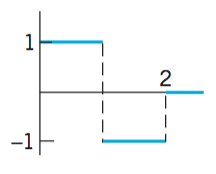
\includegraphics[width = 0.3\columnwidth]{LaplaceFig2.png}
\end{figure}
\par \textbf{Solution:}
\par You first need to express $f(t)$ as a piecewise function, then express it using Heaviside step functions:
\begin{align*}
f(t) &= \begin{cases}
1 & 0< t < 1\\
-1 & 1< t< 2\\
0 & t > 2
\end{cases}\\
\implies f(t) &= (1 - u(t-1)) - (u(t-1) - u(t - 2))\\
&= 1 - 2u(t-1) + u(t-2)\\
\intertext{Now, we can plug this into our ODE and solve via Laplace transform.}
y'' + 4y &= f(t)\\
&=  1 - 2u(t-1) + u(t-2)\\
s^2 Y(s) - sy(0) - y'(0) + 4Y(s) &= \frac{1}{s} - \frac{2e^{-s}}{s} + \frac{e^{-2s}}{s}\\
s^2 Y(s) + 4Y(s) &= \frac{1}{s} - \frac{2e^{-s}}{s} + \frac{e^{-2s}}{s}\\
Y(s) (s^2 + 4) &= \left( 1 - 2e^{-s} + e^{-2s}\right)\frac{1}{s}\\
Y(s) &= \left( 1 - 2e^{-s} + e^{-2s}\right)\frac{1}{s(s^2 + 4)}\\
\frac{1}{s(s^2 + 4)} &= \frac{A}{s} + \frac{Bs + C}{s^2 + 4}\\
1 &= As^2 + 4A + Bs^2 + Cs\\
1 &= 4A,\quad 0 = C,\quad 0 = A + B\\
A &= \frac{1}{4}\\
B&= -\frac{1}{4}\\
\frac{1}{s(s^2 + 4)} &= \frac{1}{4s} - \frac{s}{4(s^2 + 4)}\\
Y(s) &= \left( 1 - 2e^{-s} + e^{-2s}\right)\left(\frac{1}{4s} - \frac{s}{4(s^2 + 4)}\right)\\
&= \frac{1}{4s} - \frac{s}{4(s^2 + 4)} - 2e^{-s}\left(\frac{1}{4s} - \frac{s}{4(s^2 + 4)}\right) + e^{-2s}\left(\frac{1}{4s} - \frac{s}{4(s^2 + 4)}\right)\\
y(t) &= \frac{1}{4} - \frac{1}{4}\cos(2t) - 2u(t-1)\left(\frac{1}{4} - \frac{1}{4}\cos(2(t-1))\right) + \\
& \qquad u(t-2)\left(\frac{1}{4} - \frac{1}{4}\cos(2(t-2))\right)\quad\blacksquare
\end{align*}

\end{enumerate}



%----------------------------------------------------------------------------------------





\end{document}